\section{Background and Motivation}
Nuclear physics sheds light on the extremes. From the structure and processes of atomic nuclei and hypernuclei to the formation and structure of some of the largest objects in the universe, neutron stars. One of the largest obstacles to these regimes stems from our incomplete knowledge of the nuclear interation. Once a possible interaction is selected, the next obstacle is to solve for properties of many-body nuclear systems using the selected, and often complicated, interaction. Currently the popular choices for 2- and 3-body nuclear interactions come in two flavors, phenomenological and those based in Chiral Effective Field Theory ($\chi$EFT). There are a large number of methods that have been developed to solve the many-body nuclear problem, and I will be using the Auxiliary Field Diffusion Monte Carlo (AFDMC) method. One of the early methods used in nuclear physics is the Hartree-Fock (HF) method. The HF method has been used to study condensed matter systems for most of a decade \cite{hartree1928, fock1930, slater1951}, but wasn't used in nuclear physics until much later when the understanding of the nuclear interaction was improved \cite{zofka1970, gogny1986}. HF begins with the mean field approximation, meaning that inter-particle interactions are accounted for by some average interaction. The wave function is usually assumed to be a Slater determinant, which is varied to minimize the energy. This calculation is often the starting place for other more sofisticated calculations. Such is the case with AFDMC and other Quantum Monte Carlo (QMC) methods.

Other notable methods are the basis set methods such as no core shell model \cite{navratil2009,barrett2013}, the coupled-cluster method \cite{hagen2014}, and the self-consistent Green's function method \cite{dickhoff2004,soma2014}. For these methods the wave function of the nuclear system is written in terms of a truncated basis, often a harmonic oscillator basis. The momentum cutoff of the basis needs to be higher than the important momenta of the interaction that is being used, in order to do calculations in momentum space. This means however that calculations with sharp potentials (like local hard wall potentials) are difficult to do with basis set methods. They do employ techniques such as Similarity Renormalization Group \cite{hergert2016} to soften these types of interaction, which consists of applying a regulator that will smoothly cut off the high momentum dependence of hard interactions such as the local contact interaction. This allows them to decrease the number of basis functions used. One of the advantages of basis set methods is that they can use local and non-local, i.e. velocity dependent, potentials. Quantum Monte Carlo (QMC) methods, which I am using in this work, complement these basis set methods. QMC methods are currently limited to mostly local potentials\footnote{Currently, interactions that are linear in the momentum can be used. Higher order terms are treated perturbatively.} \cite{lynn2012}, but can converge for a wide variety of local Hamiltonians. Also, QMC methods do not have the momentum cutoff limits or the poor scaling with basis set size of the basis set methods.

\red{This is from my comp so maybe work it over a bit \\}
One of the most accurate QMC methods is the Green's Function Monte Carlo (GFMC) method, which has had good success calculating properties of light nuclei and nuclear matter using 2- and 3-body potentials as well as electroweak currents \cite{carlson2015}. GFMC has been used to calculate binding energies as well as excitation spectra for nuclei up to $^{12}$C with good accuracy.
\begin{figure}[h!]
   \centering
   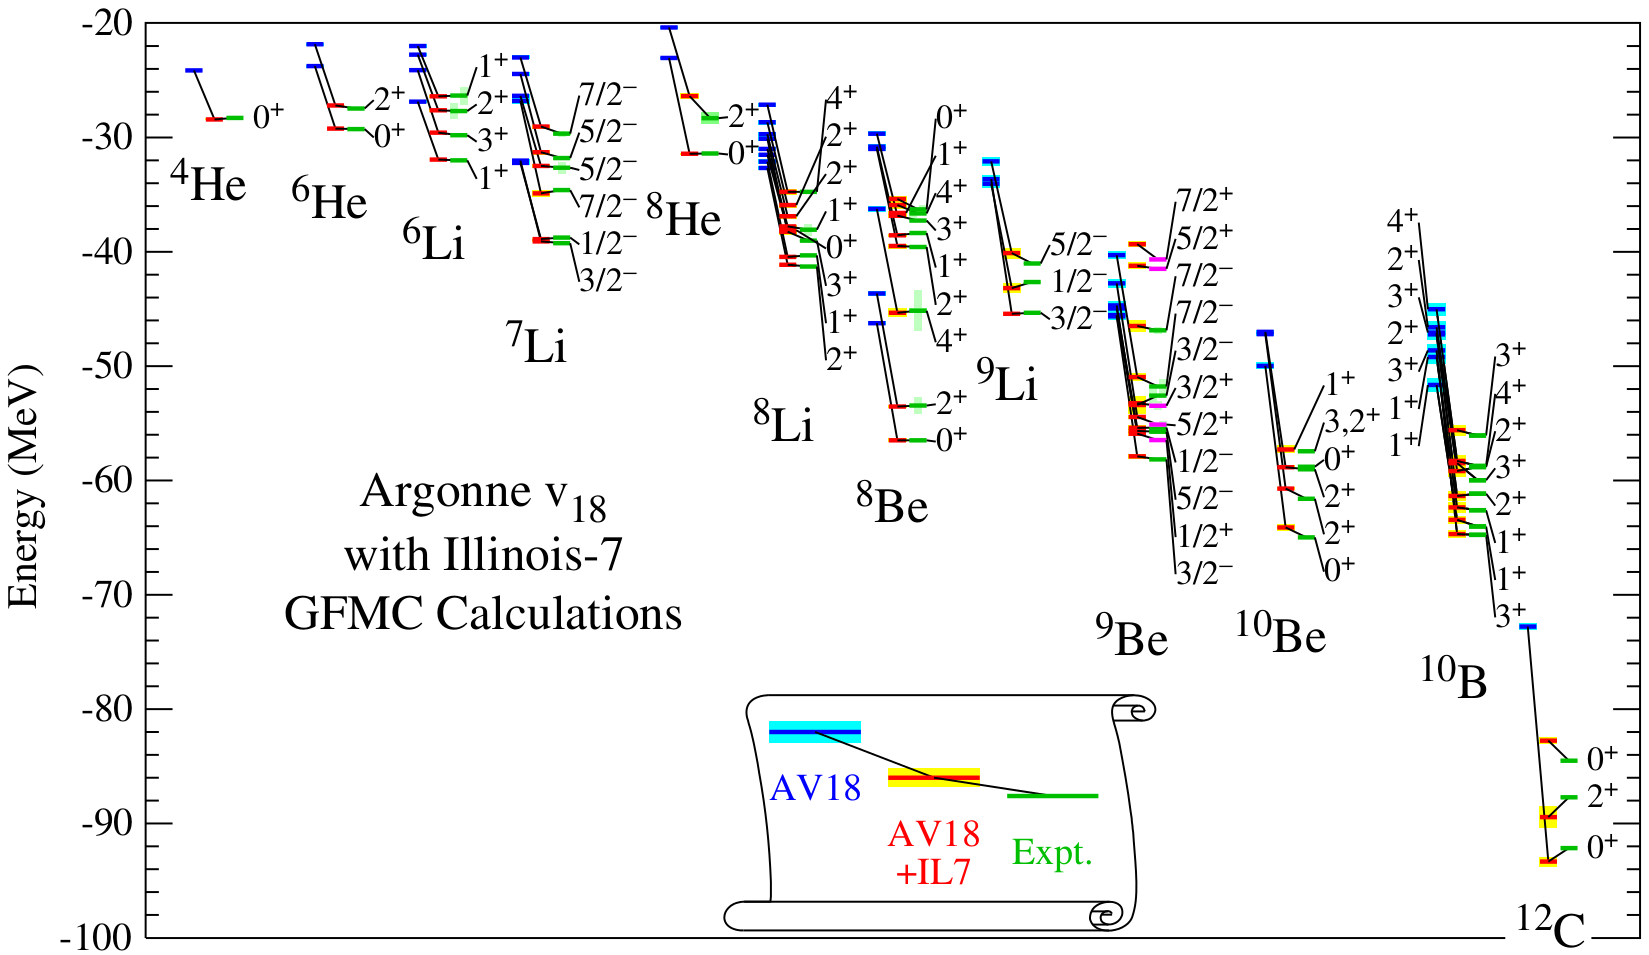
\includegraphics[width=0.8\textwidth]{figures/gfmc_energies.png}
   \caption{Ground and excited state energies calculated with GFMC calculated with the AV18 and AV18+IL7 potentials compared to experiment. Figure taken from \cite{carlson2015}.}
   \label{fig:energy_jaslin}
\end{figure}
GFMC has also been used to study electroweak current, elastic and inelastic form factors, and the neutron and symmetric nuclear matter equation of state (EOS) which have been used to study the structure of neutron stars. Nuclear calculations using the GFMC method are limited due to the explicit sum over spin states when calculating expectation values. In 1999 Schmidt and Fantoni \cite{schmidt1999} proposed the AFDMC method which is practically identical to GFMC in its Monte Carlo sampling of spatial integrals, however AFDMC uses Monte Carlo to sample the spin-isospin sums as well. Since then AFDMC has been used to study \blue{fill in gaps here with recent review by Lynn.}

\red{Add something about the awesomeness of AFDMC, show plots from Lonardoni2018 etc.}
\red{\\ Add a bit about HF and how HF, GFMC, and AFDMC all use a similar form for the wave function}

In this study, for simplicity, I have only used the AV6' phenom. potential...
\red{Mention the recent paper Ground-state properties of doubly magic nuclei from the unitary-model-operator approach with the chiral two- and three-nucleon forces, they do calculations using the Unitary-Model-Operation Aproach (UMOA) on the same light doubly-magic systems that we do but using the $\chi$EFT NN and 3N potentials with the similarity renormalization group applied (to soften them?).}
